\documentclass{article}
\usepackage{full page}
\usepackage{listings}
\usepackage{color}
\usepackage{wrapfig}

\definecolor{mygreen}{rgb}{0,0.6,0}
\definecolor{mygray}{rgb}{0.5,0.5,0.5}
\definecolor{mymauve}{rgb}{0.58,0,0.82}

\lstset{ %
  backgroundcolor=\color{white},   % choose the background color; you must add \usepackage{color} or \usepackage{xcolor}
  breakatwhitespace=false,         % sets if automatic breaks should only happen at whitespace
  breaklines=true,                 % sets automatic line breaking
  captionpos=b,                    % sets the caption-position to bottom
  commentstyle=\color{mygreen},    % comment style
  deletekeywords={...},            % if you want to delete keywords from the given language
  escapeinside={\%*}{*)},          % if you want to add LaTeX within your code
  extendedchars=true,              % lets you use non-ASCII characters; for 8-bits encodings only, does not work with UTF-8
  frame=none,                    % adds a frame around the code
  keepspaces=true,                 % keeps spaces in text, useful for keeping indentation of code (possibly needs columns=flexible)
  keywordstyle=\color{blue},       % keyword style
  language=Java,                 % the language of the code
  morekeywords={*,...},            % if you want to add more keywords to the set
  numbers=none,                    % where to put the line-numbers; possible values are (none, left, right)
  showspaces=false,                % show spaces everywhere adding particular underscores; it overrides 'showstringspaces'
  showstringspaces=false,          % underline spaces within strings only
  showtabs=false,                  % show tabs within strings adding particular underscores
  stringstyle=\color{mymauve},     % string literal style
  tabsize=2,                       % sets default tabsize to 2 spaces
  title=\lstname                   % show the filename of files included with \lstinputlisting; also try caption instead of title
}

\usepackage[pdftex]{graphicx}
\usepackage{float}
\usepackage{caption}
\usepackage{subcaption}
\lstset{language=Java}

\title{Probabilistic Reasoning Over Time}
\author{Michelle Shu}

\begin{document}
\maketitle

\section{Introduction}

In some scenarios, agents are unable to obtain complete information about their environments and must piece together their current state based on experience and partial observations. In this paper, I will describe the application of a probabilistic temporal model to a specific problem of robot localization. 

\vspace{2mm}

The premise of the problem is this: A robot is located at an unknown location on an $n$x$n$ grid. The robot can move in any of the 4 cardinal directions (North, East, South, West), but cannot detect the result of its motion or the direction it moved. Thus, if the robot tries to move into a wall, it will not move and stay in its original position, but it has no means of knowing whether it has just moved or not. The robot has only one sensor. It points downward and can tell the robot with better than chance accuracy the color of the grid square beneath it. Using this observation, along with an internal knowledge of both the map and the colors of its grid squares, the robot must infer a probabilistic distribution of its current location.

\section{A Temporal Model for the Blind Robot Problem}

An agent in an unknown environment must keep track what it knows about its current state as it explores the world. Our robot keeps track of a weighted belief state, reflecting the locations where it could possibly be at the current time point and corresponding ratings for its confidence of being in each location (likeliness of being in each location). Using probabilistic inference, the robot modifies its belief state at each discrete time point by following a transition model and a sensor model. The transition model specifies how the robot's location in the world changes with each movement. The sensor model specifies how the color of the floor at a given location is read from the sensor.

\subsection{Transition Model}

I model the changes in the robot's belief state as a first-order Markov process, in which the current belief state (at time $t$) is derived only from the information contained in the previous belief state (time $t-1$), without consideration of the earlier states that occurred before $t-1$. Figure 1 depicts a simple case of a robot on a $2$x$2$ grid. At time $t-1$, the robot believes with some set of probabilities that it is either at location $0$, $1$, $2$ or $3$. Let $P(L_{t-1} = 0)$ denote what the robot believes to be its probability of being at location $0$ during time $t-1$. 

\vspace{2mm}

In each time step, the robot moves one step in a random direction, but it is not aware of which direction it moves. All possible movements are shown in Fig.1b. It assumes that the probabilities of the direction of the last move being N, E, S, W are equivalent (all $0.25$). We use the law of conditional probability on the space of possible transitions to compute the values $P(L_t)$ for all grid locations. Computing these values for each grid square allows us to model the transition of the robot location from one time step to the next. For example, here is the computation for $P(L_t = 0)$:

\vspace{5mm}

Let $l_{t-1}$ represent all possible locations at time $t-1$.

\vspace{5mm}

$P(L_t=0) = \sum_{l_{t-1}}P(L_t=0 | l_{t-1})P(l_{t-1})$

\vspace{4mm}\hspace{17mm}$ = P(L_t=0 | L_{t-1}=0)P(L_{t-1} = 0) + P(L_t=0 | L_{t-1}=1)P(L_{t-1} = 1)  + $

\vspace{2mm}\hspace{22mm}$ P(L_t=0 | L_{t-1}=2)P(L_{t-1} = 2) + P(L_t=0 | L_{t-1}=3)P(L_{t-1} = 3) $

\vspace{4mm}$P(L_t=0) = (0.5)*P(L_{t-1} = 0) + (0.25)*P(L_{t-1} = 1) + (0.25)*P(L_{t-1} = 2) $

\vspace{5mm}

\vspace{5mm}

\begin{figure}[!htb]
\centering
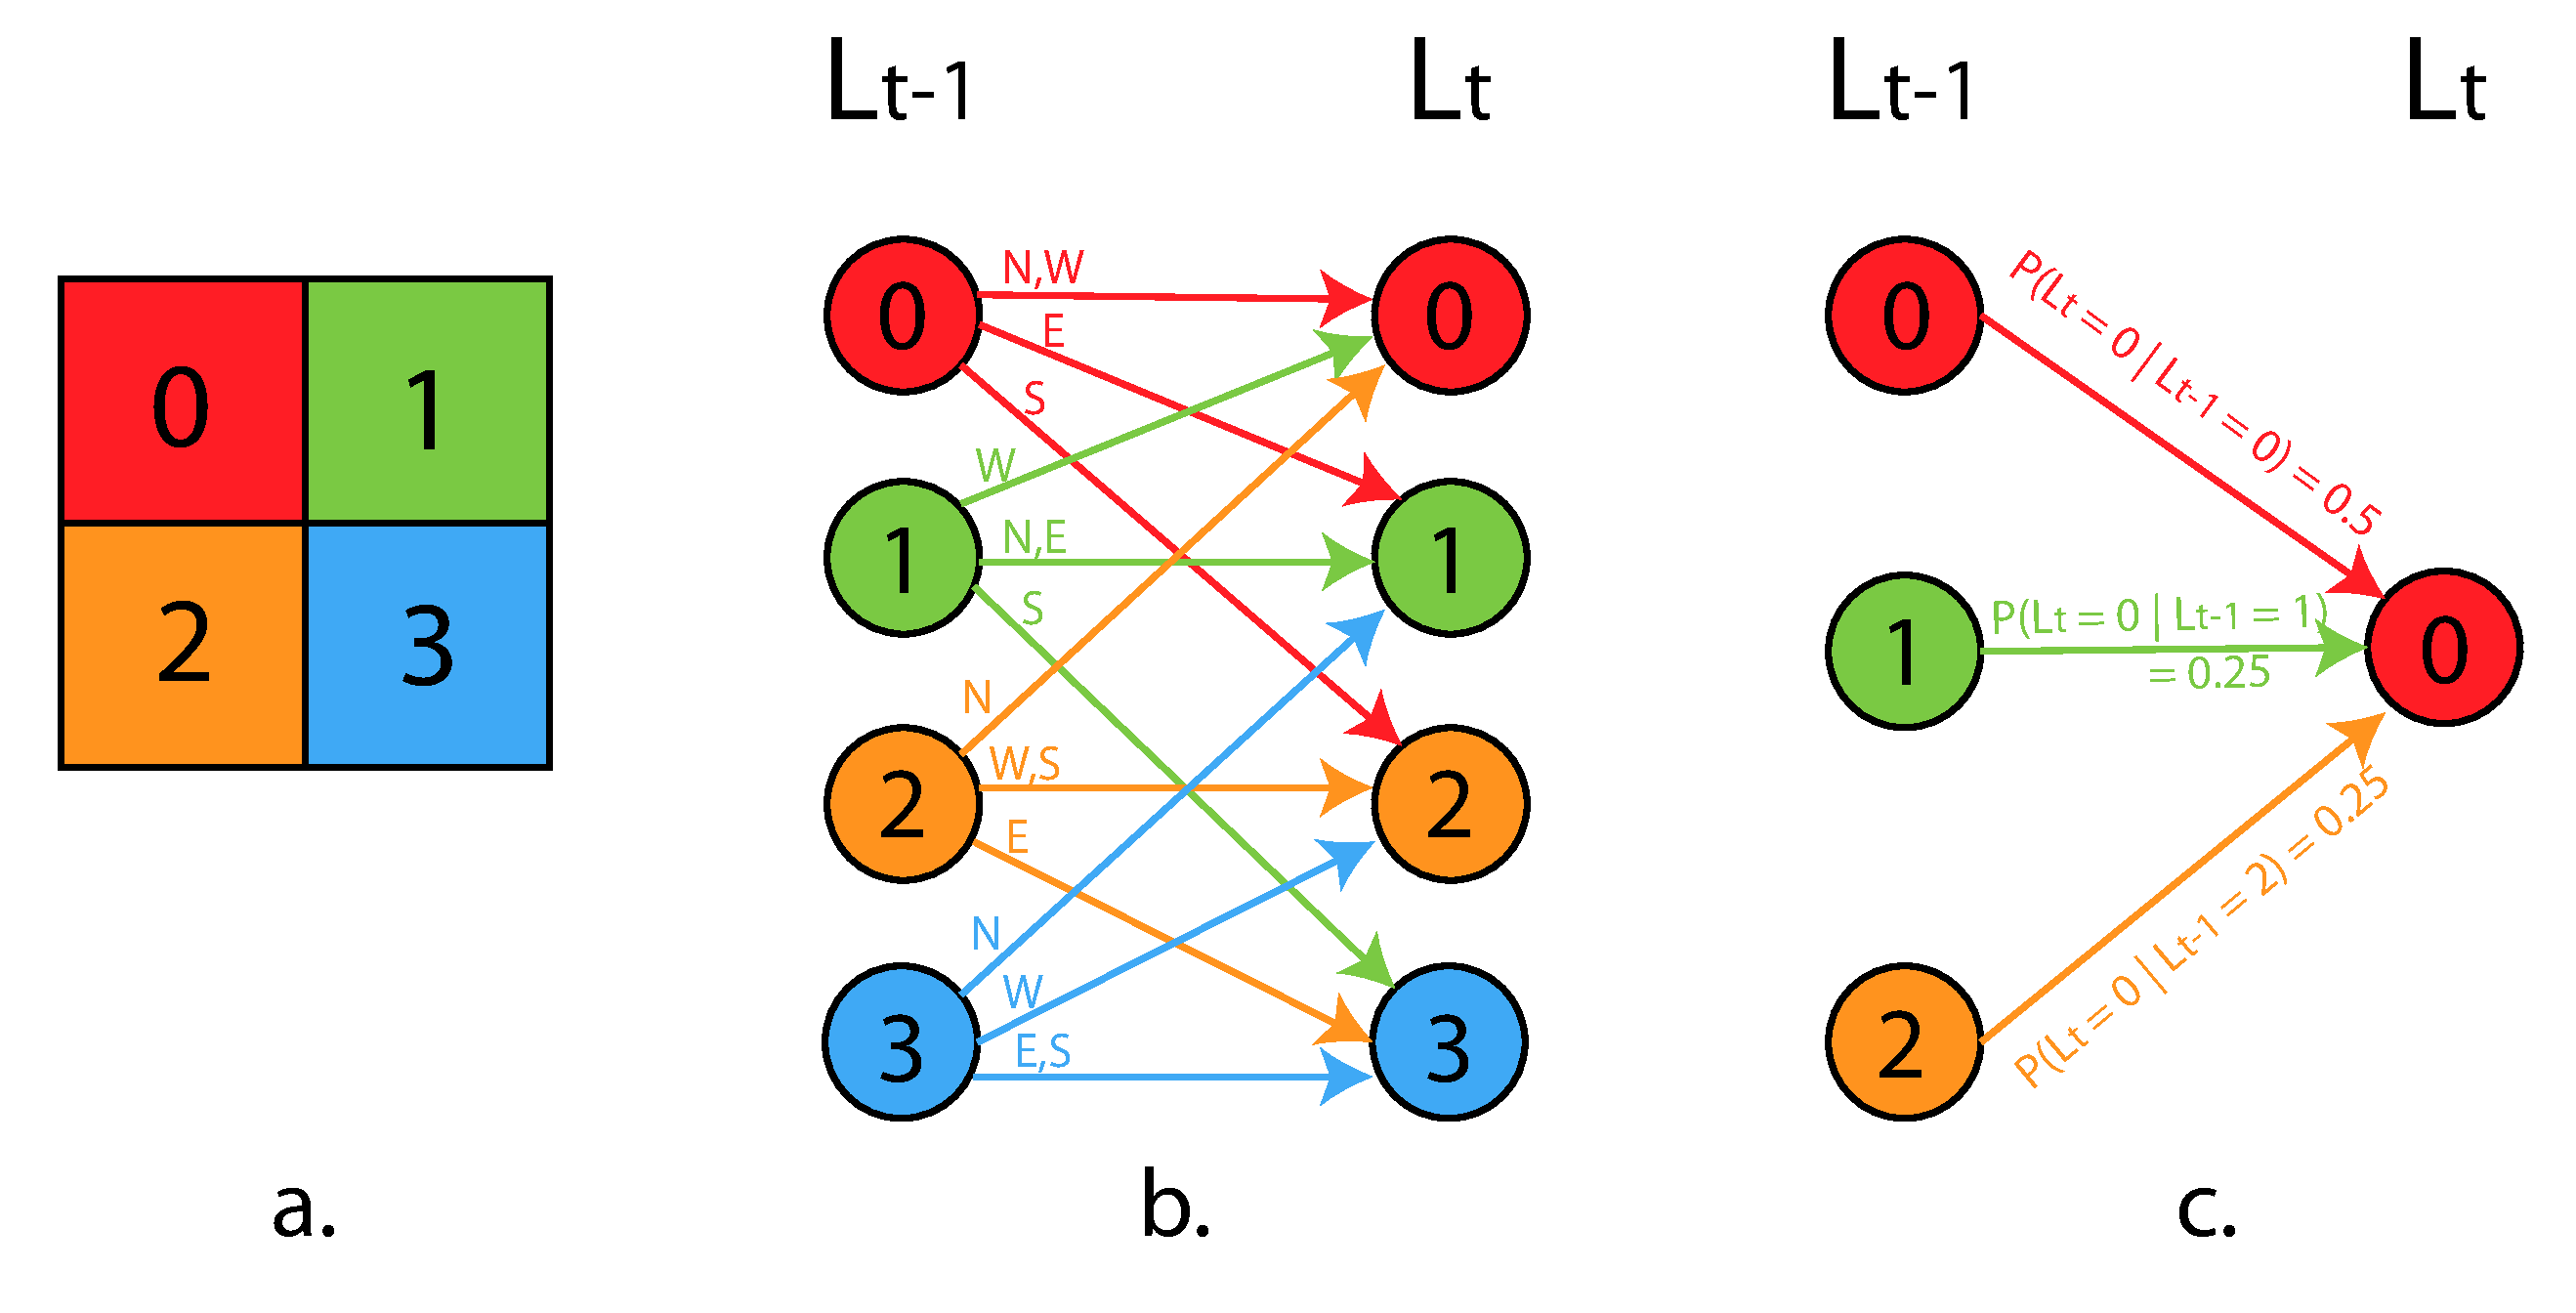
\includegraphics[scale=0.4]{transitions.pdf}
\caption{{\bf State Transition Diagram} a. A 2 x 2 colored grid on which the robot resides \hspace{1mm} b. All possible state transitions with movements in any of 4 directions \hspace{1mm} c. The conditional probabilities from all origins of movement to position 0 at time t }
\end{figure}

\subsection{Sensor Model}

We declare that each grid square can be one of four colors: Red, Green, Blue or Yellow. The robot's sensor is able to read the correct color $88\%$ of the time and reads each of the other colors (the wrong ones) $4\%$ of the time. So if the robot is currently above a blue square, the sensor would read blue with probability $0.88$, green with probability $0.04$, yellow with probability $0.04$ and red with probability $0.04$. The sensor reading at time $t$ provides evidence $e_t$ to the robot which, along with the transition model probabilities, can help it infer where it is.

The sensor evidence is a consequence of the state transition model. It is the robot's location in the world that causes the sensors to pick up the reading that they do. But the robot has no way to estimate $P(L_t | C_t)$, where $C_t$ is the color read by the sensor at time $t$. However, it can use what it knows about the accuracy of the sensor to estimate $P(C_t | L_t)$ which, turns out to be useful to know for our Bayesian temporal model. Specifically, $P(C_t | L_t) = 0.88$ if the color read matches the color of the grid square and $P(C_t | L_t) = 0.04$ if they do not match.

\section{Probabilistic Filtering}

One inference technique performed on temporal probabilistic models is called {\bf filtering}. Filtering is the process of computing a belief state based on all evidence and experience gathered up until the current time point. I implement a filtering algorithm that maintains a belief state consisting of the estimated probabilities of the robot being in each possible position on the grid. The belief state will be incrementally updated as the robot moves by applying the transition model and the sensor model in conjunction.

Here is the structure of the filtering model (based on the figure in Russell and Norvig), which shows causal relationships between states and evidence:

\begin{figure}[!htb]
\centering
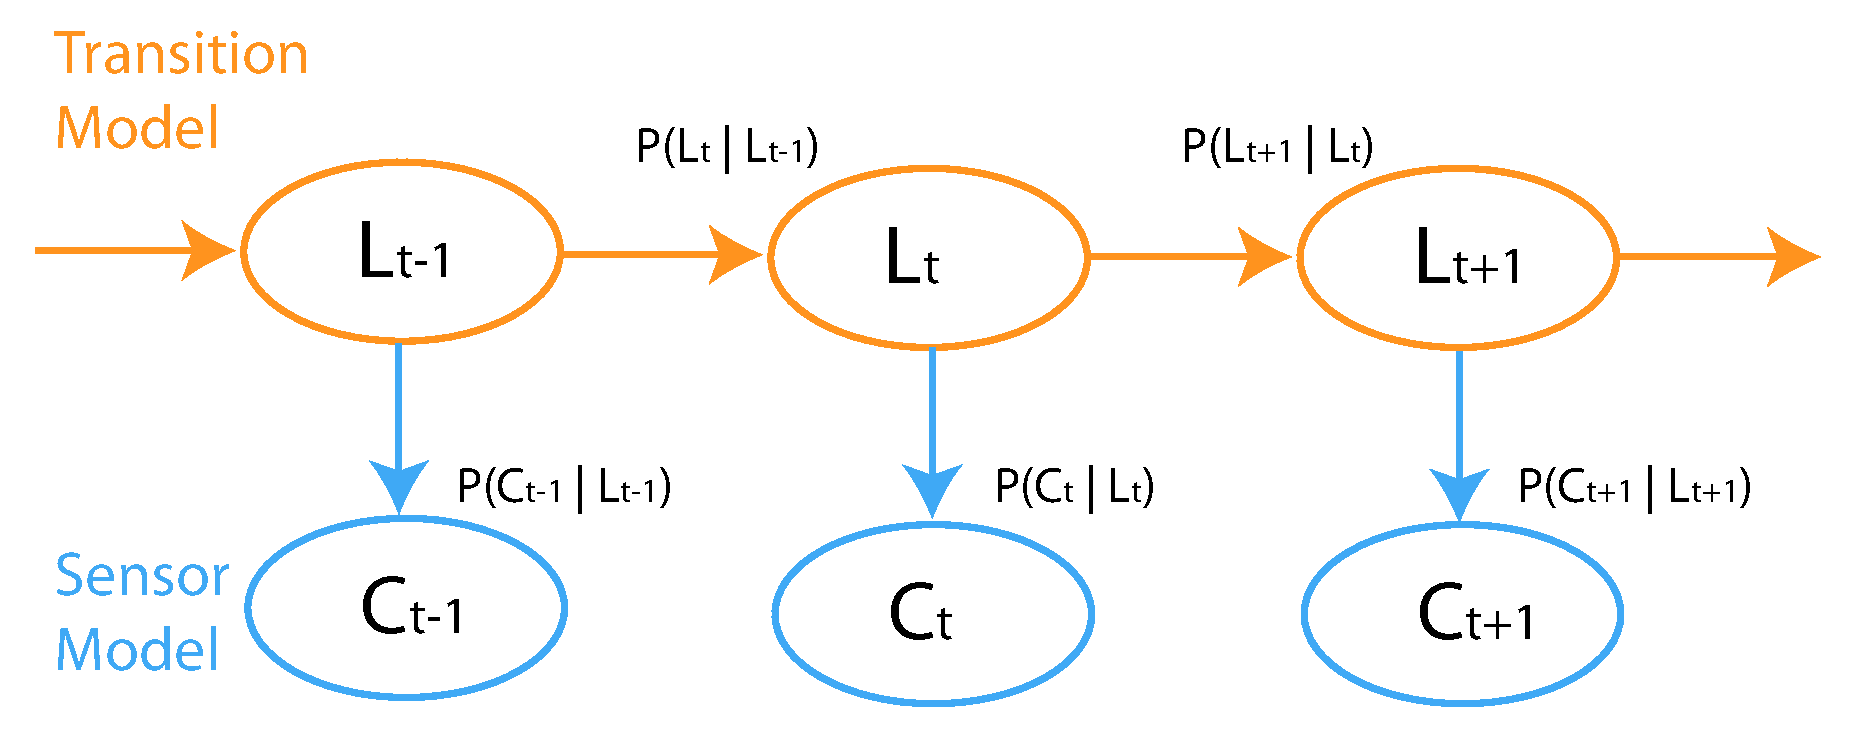
\includegraphics[scale=0.55]{bayesiannetwork.pdf}
\caption{{\bf Bayesian Network Structure} The relationship between the transition model and sensor model}
\end{figure}

The filter produces a conditional distribution of the robot's location at time $t$ given the prior distribution and the evidence observed in prior steps. In other words, we define the following update step (Russell and Norvig) derived from Bayes' rule and the Markov assumption to compute the values $P(L_t | C_{1:t})$:

\vspace{5mm}

$P(L_t | C_{1:t}) = \alpha P(C_t | L_t) \sum_{l_{t-1}} P(L_t | l_{t-1})P(l_{t-1} | C_{1:t-1})$ 

\vspace{5mm}

The factor inside the summation is derived from applying the transition model and the factor outside is derived from the sensor model. $\alpha$ is a normalization factor which ensures that the probabilities sum to 1.

\section{Code Design}

I partitioned my code into the following classes:

\begin{itemize}
\item \verb`GridWorld.java`: Contains layout and colors of grid space that robot is on, and functions used to read this in from a text file format.
\item \verb`Sensor.java`: The sensor collects readings of grid square colors from the world that the robot is in. It knows the ground truth location and movements of the robot in order to produce readings, but this is information hidden from the robot itself.
\item \verb`Robot.java`: Stores belief state of robot and conducts updates using transition and sensor models.
\item \verb`Matrix.java`: Utility class containing general implementations of matrix operations (e.g. normalizing)
\item \verb`WorldView.java`: A JavaFX view that shows the robot's true location and belief state. It also allows us to step through movements and belief state updates with button callback.
\end{itemize}

\section{Implementation}

\subsection{Grid Representation (GridWorld)}

Grid layouts are read in from a text file of comma-delimited values presented in the same orientation that they would be laid out as grid squares. Each value can be any color value from the set \{R, G, B, Y\} or a period (.) to represent an obstacle. The example 5x5 grid I will be using is represented in text format as the following:

\vspace{5mm}

{\setlength{\parindent}{0cm}
R,G,B,Y,B\\
.,R,R,G,G\\
.,.,B,.,Y\\
Y,Y,B,.,R\\
B,G,G,.,Y\\
}

This is read in and stored as a 2-dimensional char array by \verb`loadGraphFromFile` in \verb`GridWorld.java`, while also tallying the number of non-obstacle spaces.

\begin{lstlisting}
private void loadGridFromFile(String filename, int w, int h) {
	this.width = w;
	this.height = h;
	this.colors = new char[height][width];
	this.validSquares = 0;
	
	BufferedReader br = null;
	try {
		br = new BufferedReader(new FileReader(filename));
		String[] row;
		for (int i = 0; i < height; i++) {
			row = br.readLine().split(",");
			for (int j = 0; j < width; j++) {
				colors[i][j] = row[j].trim().toCharArray()[0];
				if (! isObstacle(i, j)) {
					validSquares++;
				}
			}
		}
	} catch (IOException e) {
		e.printStackTrace();
	} finally {
		try {
			if (br != null) br.close();
		} catch (IOException ex) {
			ex.printStackTrace();
		}
	}
}
\end{lstlisting}

\verb`GridWorld.java` also includes some auxiliary functions that are used to determine whether a specific location on the grid is in bounds or an obstacle and to get the locations of the neighbors of any grid cell. The \verb`getAdjacentLocs` function handles adjacent walls and obstacles by using the current location itself as a neighbor in these instances. This reflects the robot's behavior of staying in the same spot when it tries to move into an invalid location. 

\begin{lstlisting}
public boolean isObstacle(int i, int j) {
	return colors[i][j] == '.';
}

public boolean inBounds(int i, int j) {
	return !(i < 0 || j < 0 || i >= height || j >= width);
}

public int[][] getAdjacentLocs(int i, int j) {
	// Get the 4 adjacent locations to (i, j) from directions N, E, S, W
	// If the neighbor is edge of board or obstacle, replace with (i, j)
	int[][] adjacentLocs = new int[4][2];
	int index = 0;
	for (int[] dir: directions) {
		if (inBounds(i + dir[0], j + dir[1]) && ! isObstacle(i + dir[0], j + dir[1])) {
			adjacentLocs[index][0] = i + dir[0];
			adjacentLocs[index][1] = j + dir[1];
		} else {
			adjacentLocs[index][0] = i;
			adjacentLocs[index][1] = j;
		}
		index++;
	}
	return adjacentLocs;
}
\end{lstlisting}

\subsection{Sensor}

The \verb`Sensor` class simulates the operation of an actual sensor of the robot. It collects readings from the actual world, so this class is "aware" of the robot's real location. When the robot collects the readings from the sensor, it will only receive a color with no additional information, and that color will only be accurate $88\%$ or P\_CORRECT\% of the time. Each time \verb`getNextReading` in \verb`Sensor.java` is called by the robot, two things will happen: the robot will move in a random direction and the result of an imperfect sensor reading from the new location will be returned.

\vspace{5mm}

\begin{lstlisting}
public Sensor(GridWorld g) {
	this.grid = g;
	this.rand = new Random();
	// Start the robot out in a random position on the board
	this.x = rand.nextInt(grid.width);
	this.y = rand.nextInt(grid.height);
}

// Get imperfect sensor reading
public char getNextReading() {
	move();
	char correctReading = grid.colors[y][x];
	if (rand.nextDouble() < P_CORRECT) {
		// Return the correct color certain percentage of the time
		return correctReading;
	} else {
		char wrongReading = colors[rand.nextInt(colors.length)];
		while (wrongReading == correctReading) {
			wrongReading = colors[rand.nextInt(colors.length)];
		}
		return wrongReading;
	}
}

// Move the robot in a random direction
public void move() {
	int[] dir = directions[rand.nextInt(directions.length)];
	if (grid.inBounds(y + dir[0], x + dir[1]) && 
			! grid.isObstacle(y + dir[0], x + dir[1])) {
		y += dir[0];
		x += dir[1];
	}
}
\end{lstlisting}

\subsection{Filtering Algorithm (Robot)}

The \verb`Robot.java` class maintains the robot's probabilistic belief state. When the \verb`update` method is called on the robot, it gets another sensor reading and updates revises its probability distribution of its current location. To accomplish this, the robot first computes the transition update on its prior belief state and then modifies this by multiplying the sensor update. 

\begin{lstlisting}
public Robot(GridWorld g) {
	this.grid = g;
	this.sensor = new Sensor(grid);
	this.belief = new double[grid.height][grid.width];
	// Initialize belief state with uniform probabilities
	Matrix.setAll(belief, grid, 1.0 / (grid.validSquares));
}

public void update() {
	// Move robot and detect next color from sensor
	char color = sensor.getNextReading();
	// Update belief state
	belief = getSensorUpdate(color, getTransitionUpdate());
}
\end{lstlisting}

\vspace{5mm}

\begin{lstlisting}
private double[][] getTransitionUpdate() {
	double[][] newBelief = new double[grid.height][grid.width];
	for (int i = 0; i < grid.height; i++) {
		for (int j = 0; j < grid.width; j++) {
			if (! grid.isObstacle(i, j)) {
				int[][] adjacentLocs = grid.getAdjacentLocs(i, j);
				newBelief[i][j] = Matrix.getAverage(belief, adjacentLocs);
			} else {
				newBelief[i][j] = 0;
			}
		}
	}
	return newBelief;
}

// Add sensor evidence factor to transition update
private double[][] getSensorUpdate(char color, double[][] transitionUpdate) {
	double[][] newBelief = new double[grid.height][grid.width];
	for (int i = 0; i < grid.height; i++) {
		for (int j = 0; j < grid.width; j++) {
			if (! grid.isObstacle(i, j)) {
				if (grid.colors[i][j] == color) {
					newBelief[i][j] = transitionUpdate[i][j] * Sensor.P_CORRECT;
				} else {
					newBelief[i][j] = transitionUpdate[i][j] * Sensor.P_INCORRECT;
				}
			} else {
				newBelief[i][j] = 0;
			}
		}
	}
	Matrix.normalize(newBelief);
	return newBelief;
}
\end{lstlisting}

The robot update functions rely on two helper functions from the matrix class. The \verb`getAverage` function takes the average of the values in given locations in the matrix. This is used to compute the sum of conditional probabilities used in the transition model (essentially the average of probabilities in 4 locations returned by \verb`getAdjacentLocs`).

\begin{lstlisting}
public static double getAverage(double[][] matrix, int[][] locs) {
	double sum = 0.0;
	for (int l = 0; l < locs.length; l++) {
		int[] loc = locs[l];
		sum += matrix[loc[0]][loc[1]];
	}
	return (sum / (double) locs.length);
}
\end{lstlisting}

The \verb`normalize` method normalizes the probability values in the belief state matrix so that they sum to 1.

\begin{lstlisting}
public static void normalize(double[][] matrix) {
	// First pass: take sum of all values in matrix
	double sum = 0;
	for (int i = 0; i < matrix.length; i++) {
		for (int j = 0; j < matrix.length; j++) {
			sum += matrix[i][j];
		}
	}
	// Second pass: divide all values by sum
	for (int i = 0; i < matrix.length; i++) {
		for (int j = 0; j < matrix.length; j++) {
			matrix[i][j] /= sum;
		}
	}
}
\end{lstlisting}


\section{Sample Output}

The following 4 pages show an example of how the robot's belief state changes as it proceeds to move in random directions in its colored grid world. The opacity of the grid colors are proportional to the entries in the robot's belief state (i.e. The more confident the robot is that is located at a particular position, the darker the color of the square.) The numerical belief state probabilities are displayed to the right of the figures. The transparent circle indicates the true location of the robot as it navigates through the grid.

This example is a simple one, as the robot only moves through the right column of the grid and sometimes stays in the same spot for multiple moves. However, due to its simplicity, I can easily make some observations that verify that the algorithm is working as expected. Here are several things to observe about the robot's inference:






The graphical user interface I am using is based in the appendix.

\begin{figure}[H]
\centering
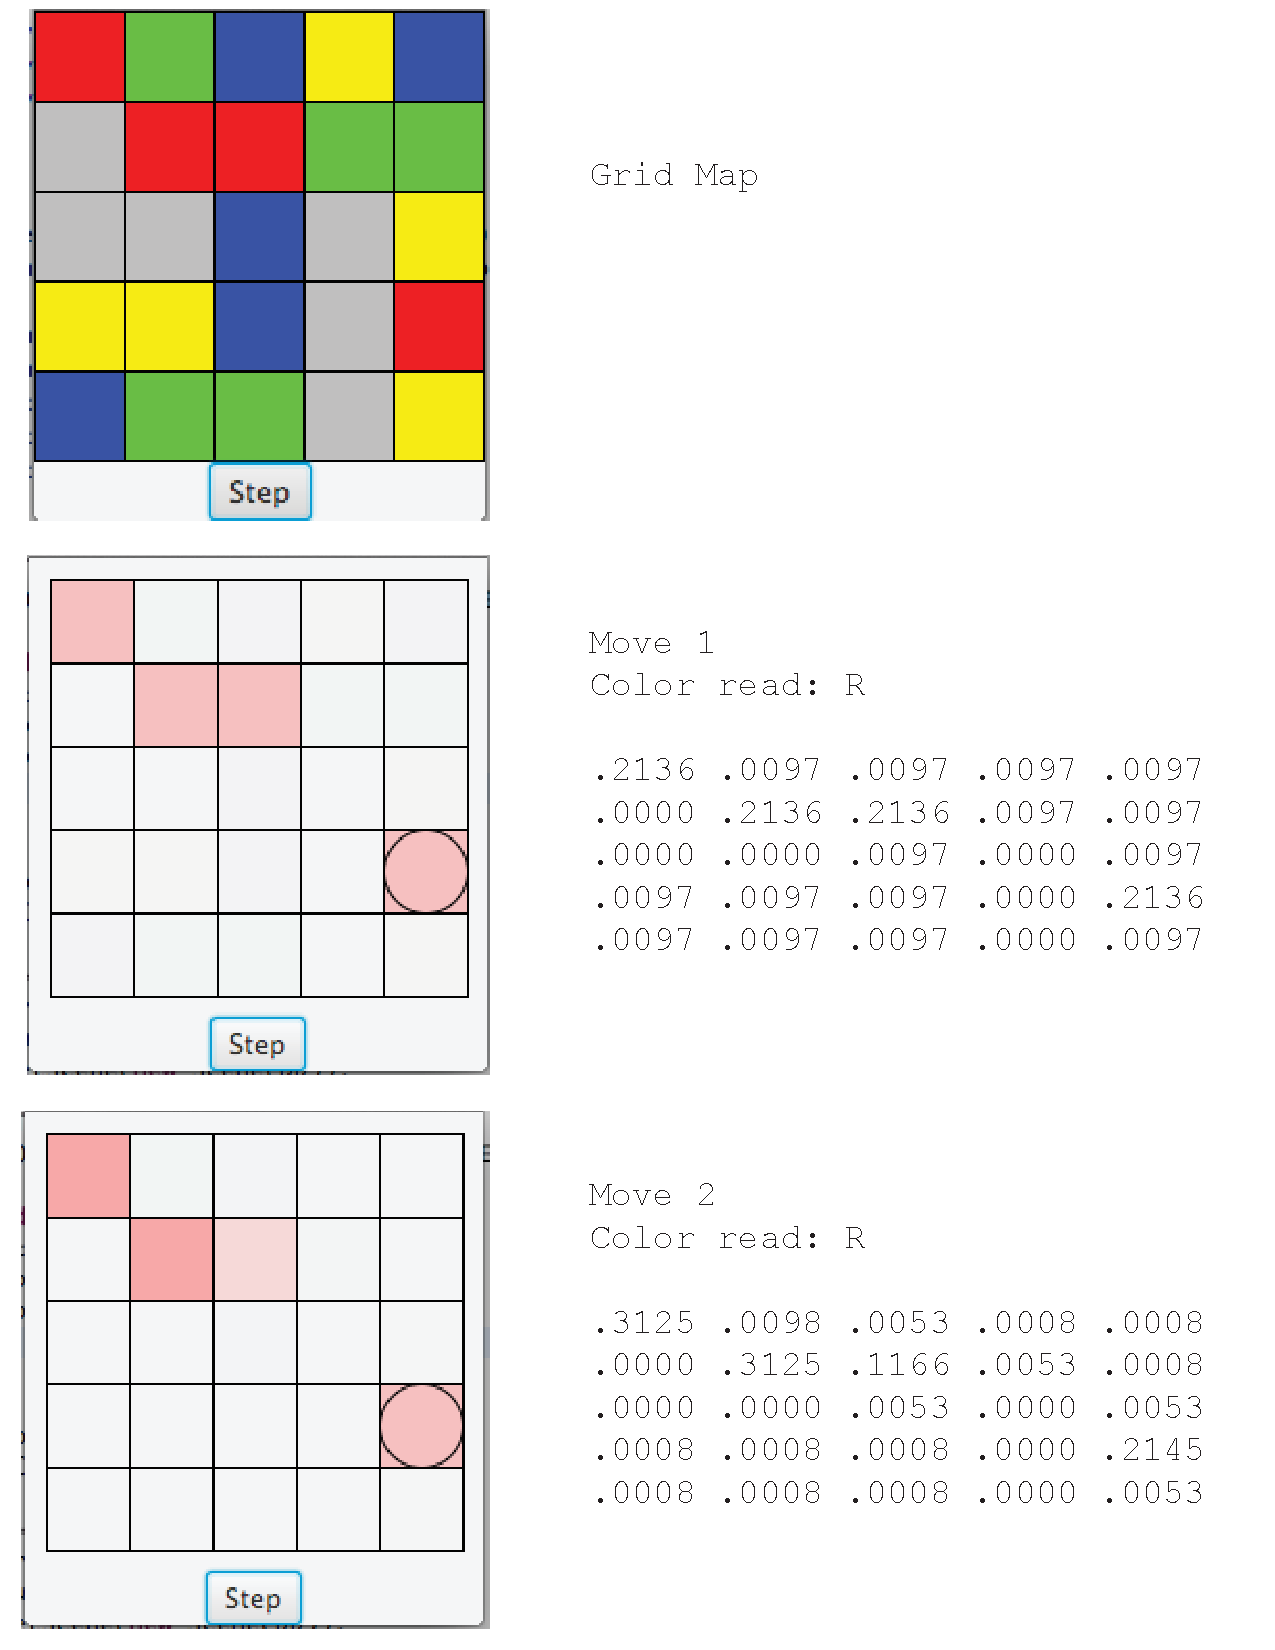
\includegraphics[scale=0.8]{example1.pdf}
\end{figure}

\begin{figure}[H]
\centering
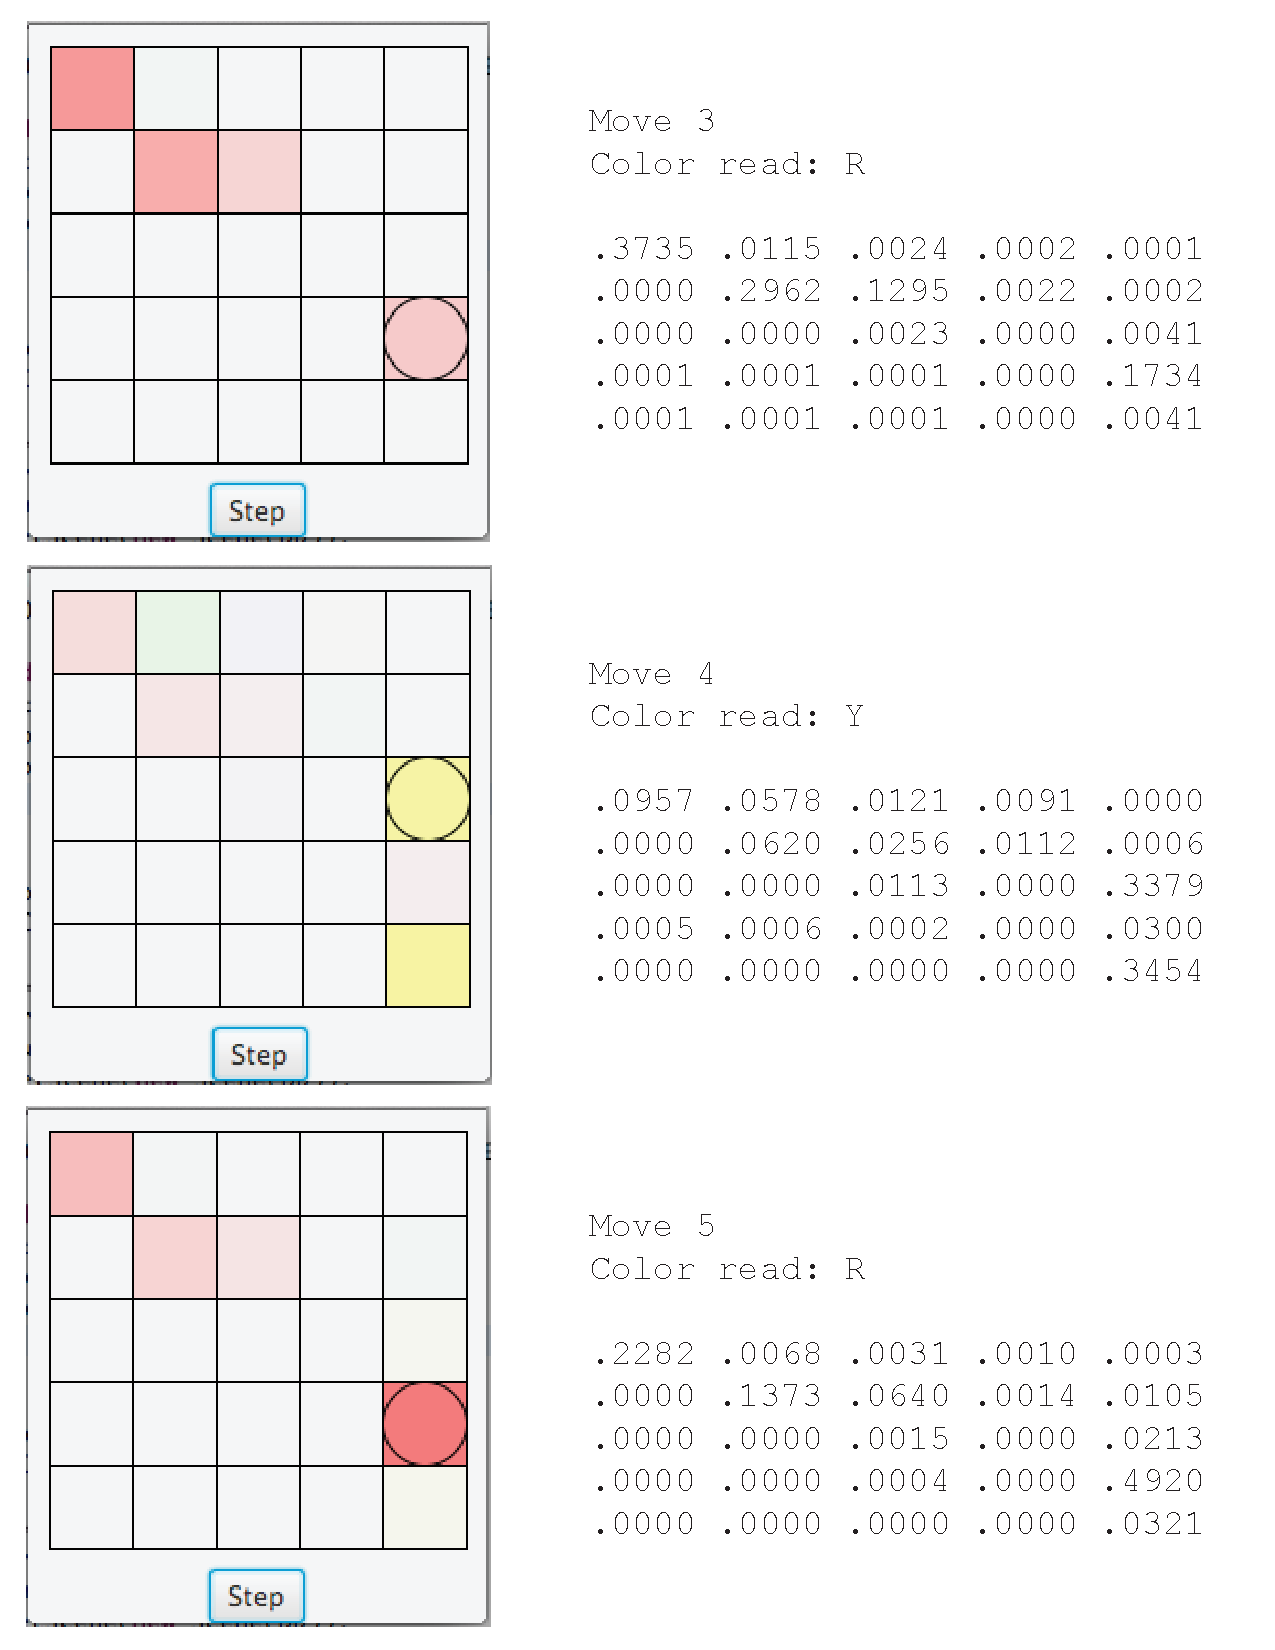
\includegraphics[scale=0.8]{example2.pdf}
\end{figure}

\begin{figure}[H]
\centering
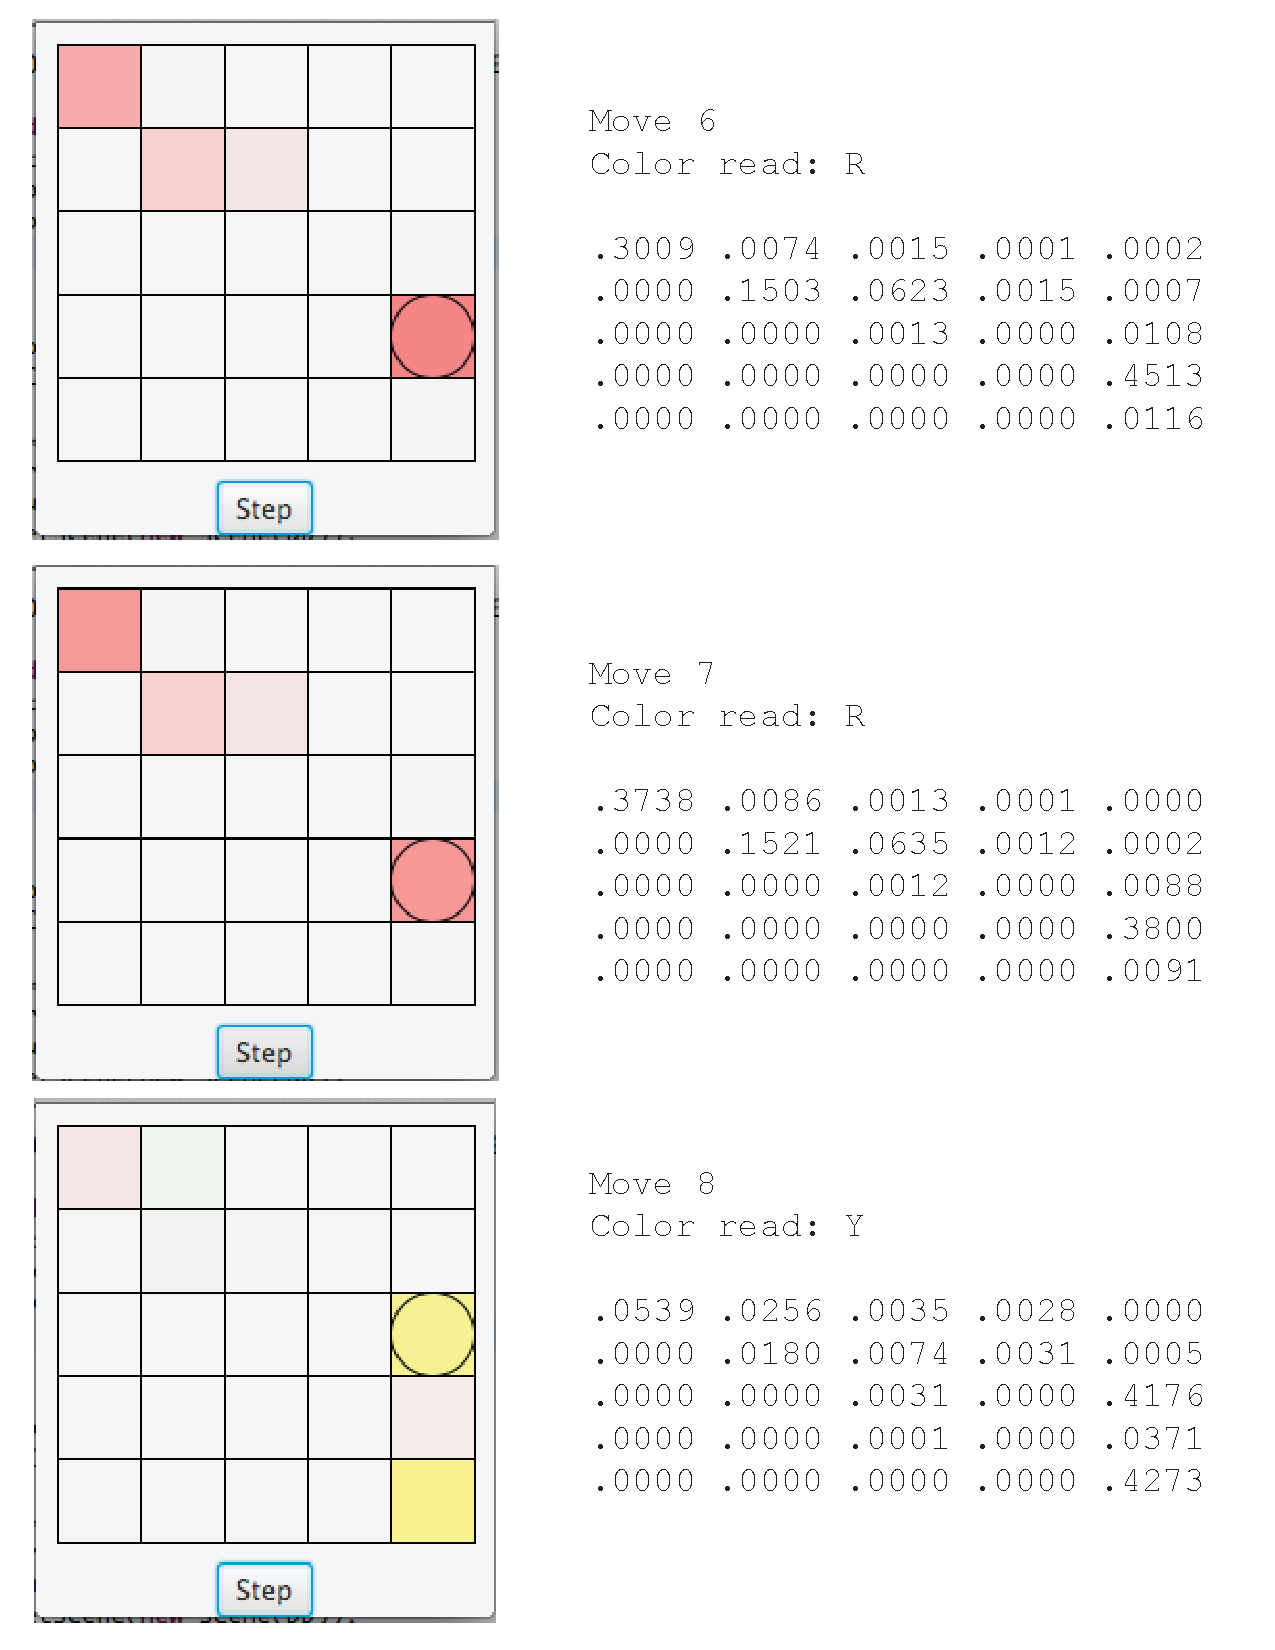
\includegraphics[scale=0.8]{example3.pdf}
\end{figure}

\begin{figure}[H]
\centering
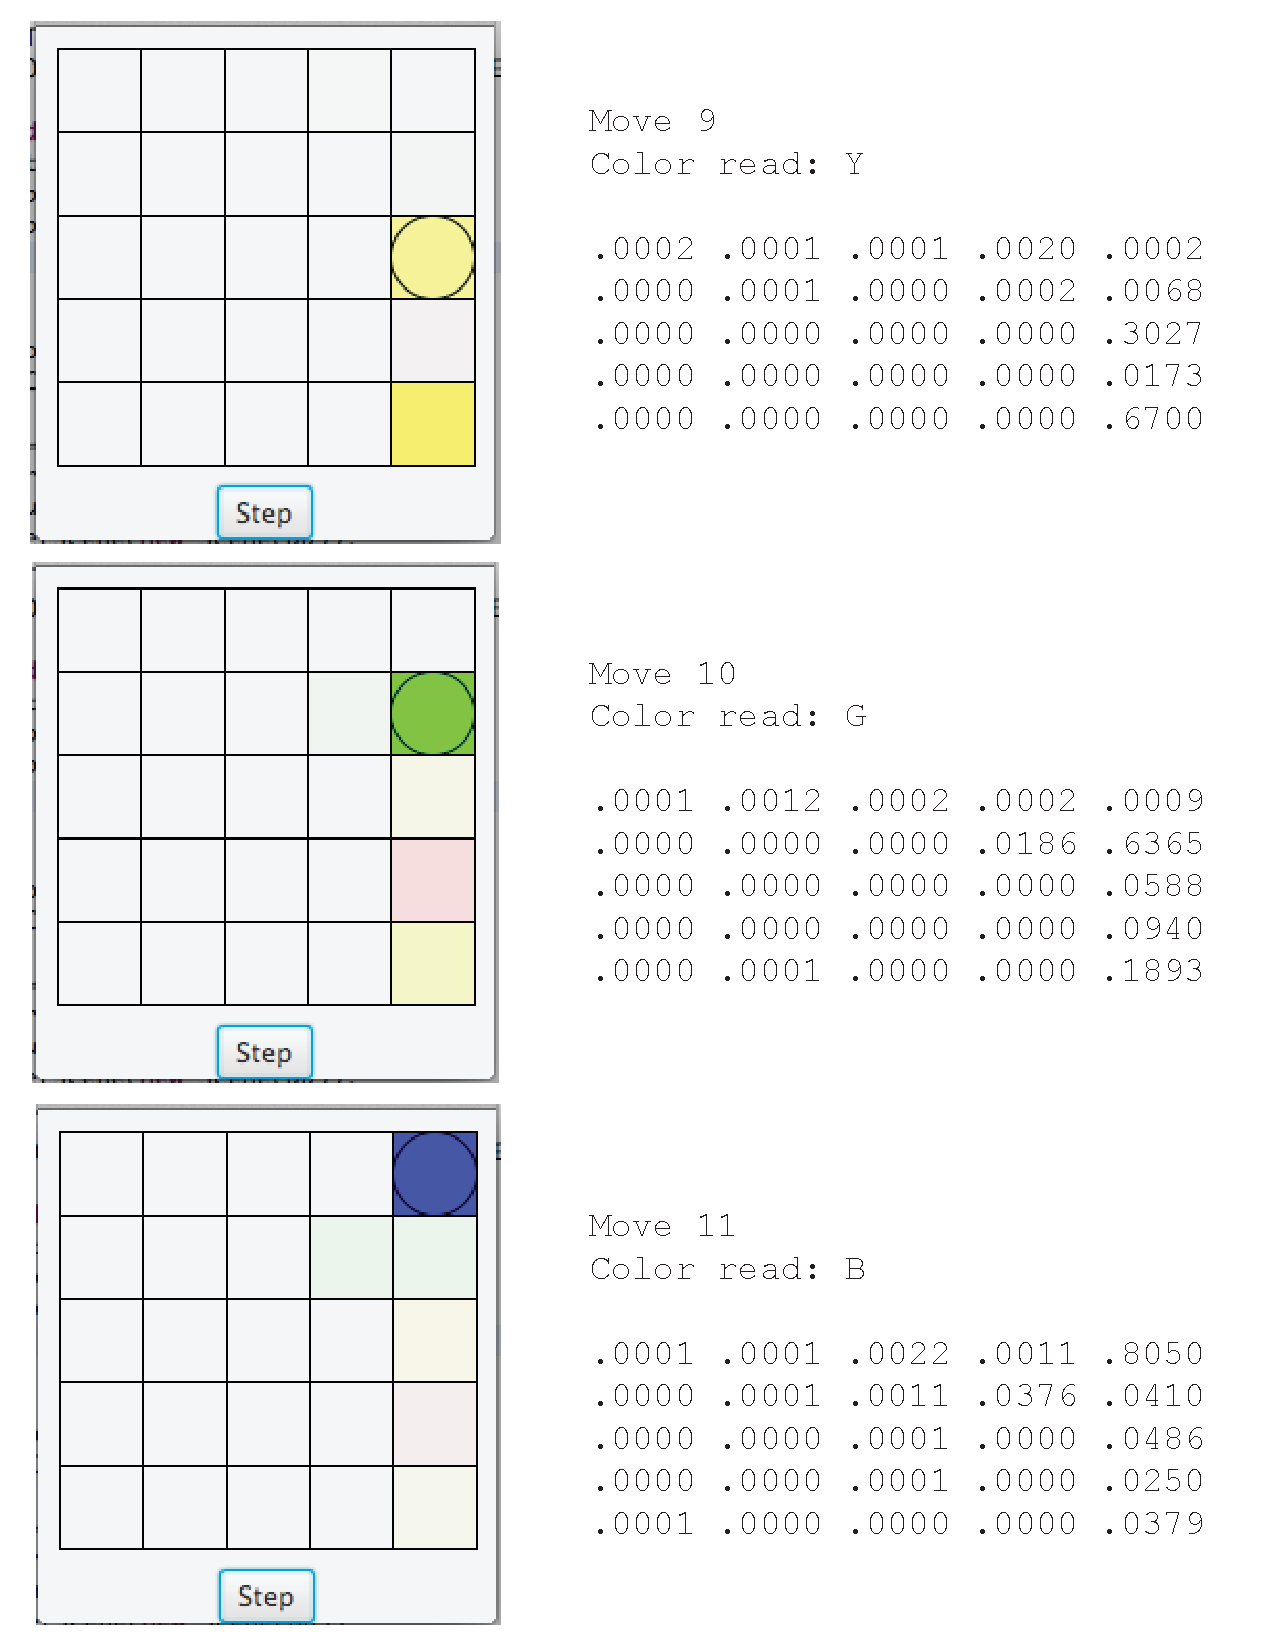
\includegraphics[scale=0.8]{example4.pdf}
\end{figure}

\newpage

\begin{figure}[H]
\centering
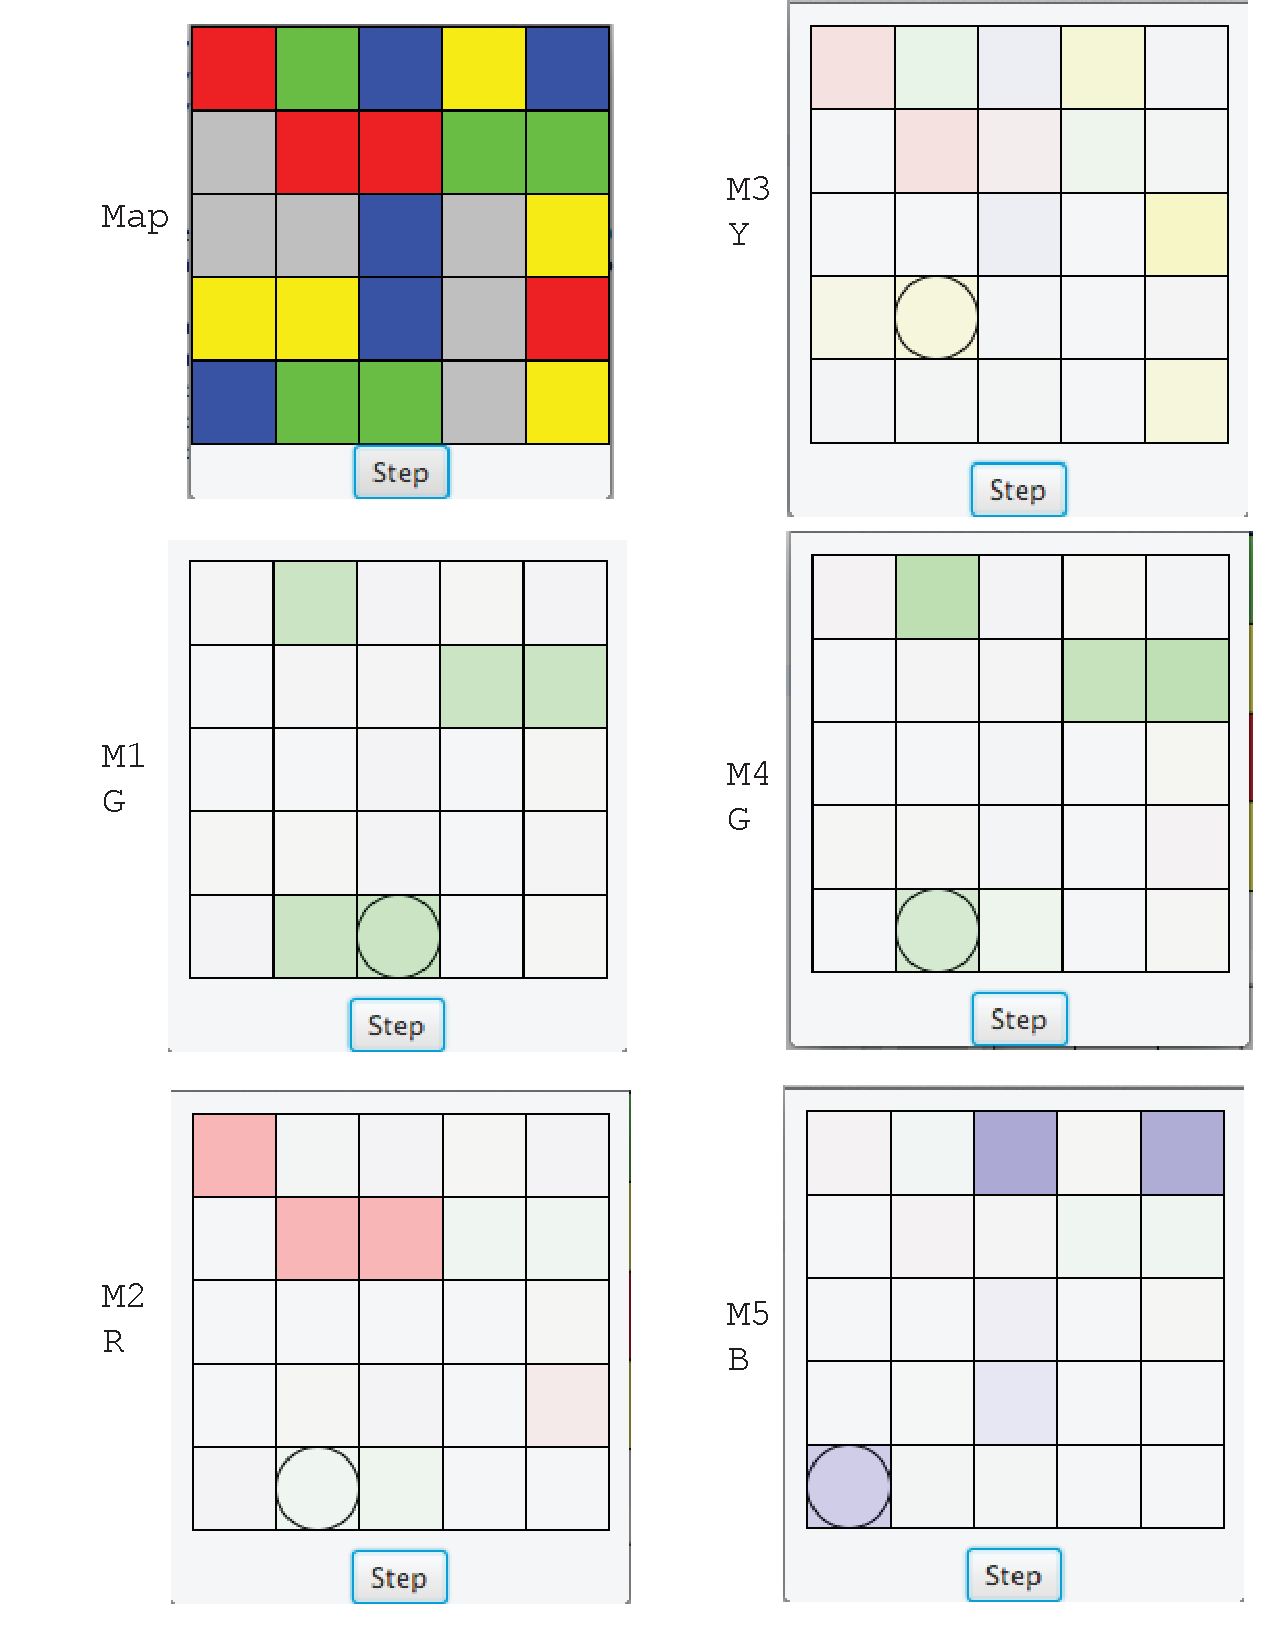
\includegraphics[scale=0.8]{exampleb.pdf}
\end{figure}

\vspace{100cm}
\section{References}
Stuart Russell and Peter Norvig. "Artificial Intelligence: A Modern Approach" 3 ed. 2010.

\section{Appendix}




\end{document}